%\vspace{-2pt}
\section{Graph-based Try-Catch Necessity Checking Model}
\label{detect:sec}

\begin{figure}[t]
	\centering
	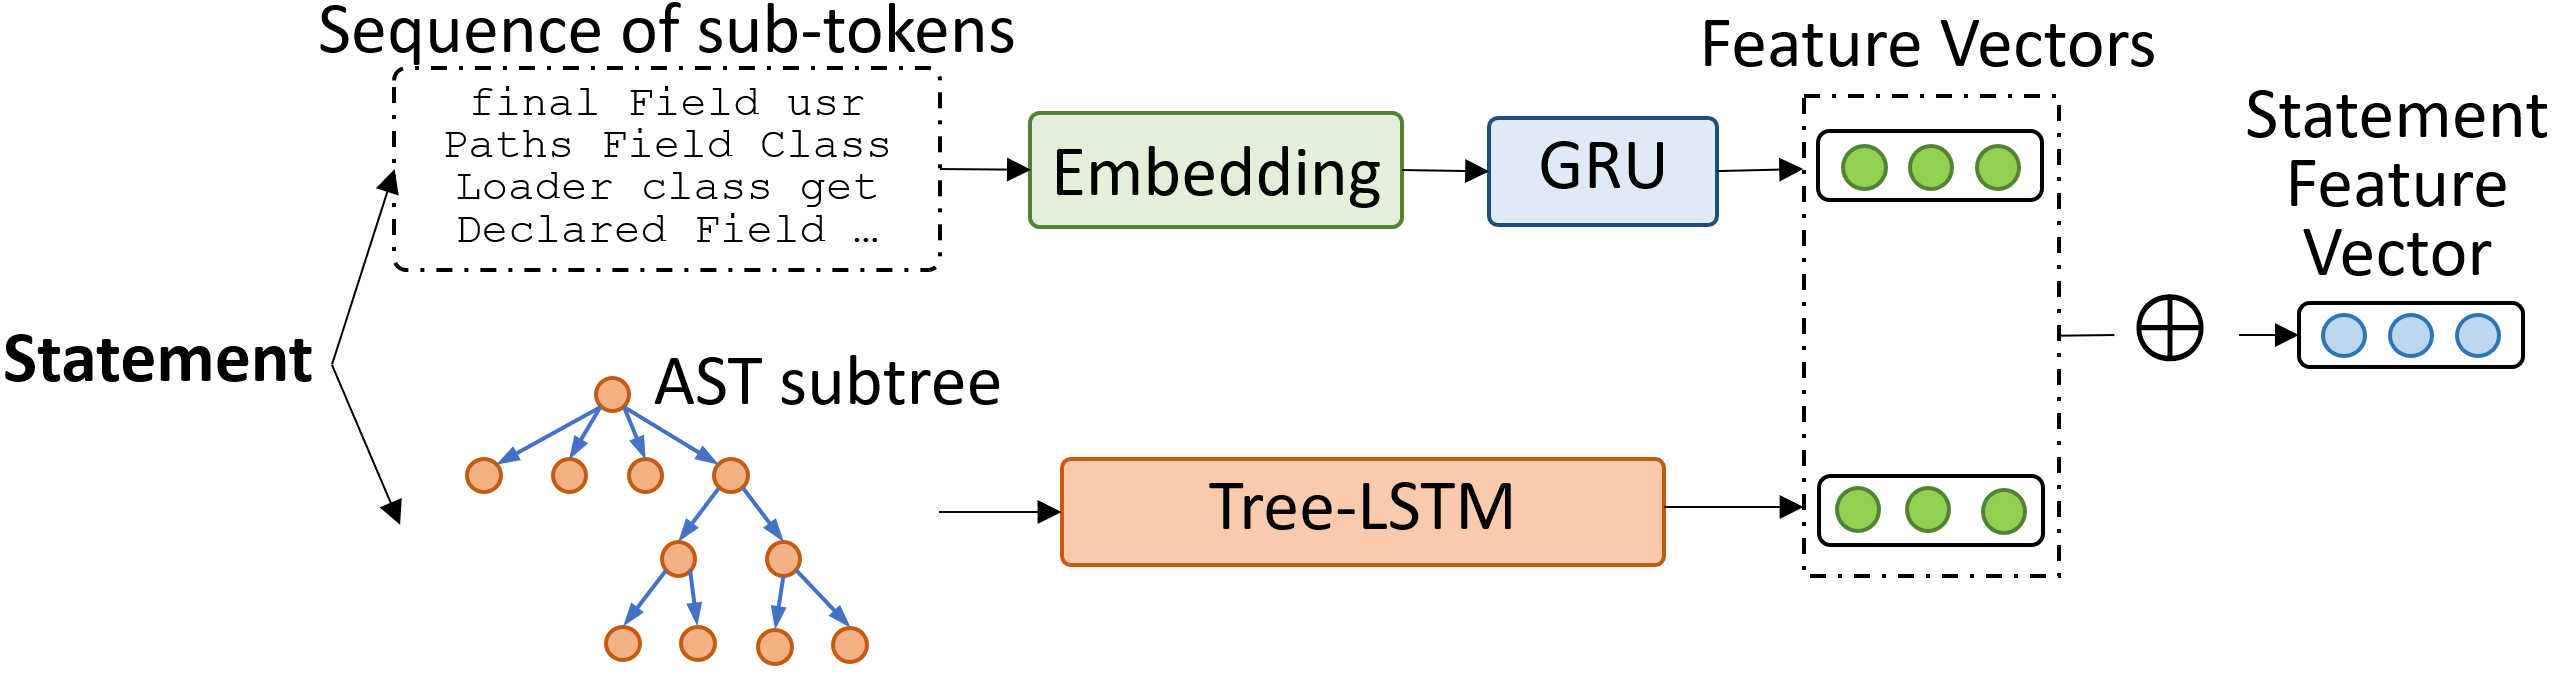
\includegraphics[width=3.2in]{features.png}
        \vspace{-0.08in}
	\caption{Code Representation Learning for Statement}
%        \vspace{-0.05in}
	\label{fig:feature}	
\end{figure}

%Tien
This section describes our graph-based {\xblock} model. We first
explain how we build the context-aware representation learning for the
given code, and then how we use such learned vectors for the detection
of the presence of \code{try-catch} block using R-GCN~\cite{yi}.

%^Feature-Attention GCN model (FA-GCN)~\cite{FAGCN} for VD. The
%rationale is that FA-GCN can deal well with the graphs with sparse
%features (not all the statements share the same properties), and
%potentially noisy features in a PDG.

%Removed this
%The key difference between FA-GCN and the traditional GCN is the way
%of computing feature representation vector $x_{V}$. While traditional
%GCN generates vector representations for each feature $x_{V,i}$, and
%summarizes them into one vector, FA-GCN enables the treatment for
%important nodes and the impacts of them on the surrounding nodes. This
%works well for the VD problem, where during training, we know the {\em
%  fixed statements} and relevant ones. By putting all features of a
%node $v$ into a sequence, FA-GCN uses a Bi-directional
%LSTM~\cite{huang2015bidirectional} to learn the hidden layer for each
%feature $x_{v,i}$ and then uses an attention layer to learn the weight
%for that feature. Then, for each node $v$, the attention-based vector
%representation is computed by merging the same feature from the
%surrounding nodes with the weights, and the same feature of the node
%$v$ into a final representation vector.



%In {\tool}, we use a graph-based deep learning approach to do the classification for vulnerability detection in order to analyzing both the code structure and context. {\tool} takes the code method as input and generate a classification result within \textit{vulnerable} and \textit{non-vulnerable} two categories which we use as the vulnerability detection. As for the specific graph-based deep learning approach, we use the Feature-attention GCN model (FA-GCN) \cite{} in {\tool}. As mentioned in key ideas section, {\tool} is proposed to using a graph-based model to do the vulnerability detection with sub-graph and node features as interpretation. To achieve this goal, FA-GCN model is a good choice that based on a feature-attention graph convolution learning framework that could be used to analyze graphs with noisy and sparse node features.

%Within FA-GCN, when it accept a graph $G_N=(V,E)$ as input, where $V$ is the node set that each node in this set has a feature representation vector $x_V$ and $E$ is the edge set, FA-GCN model will come up with a summzerized $N\times D$ feature matrix where $N$ is the total number of statements and $D$ is the total number of features and a label function on nodes or the whole graph $f:V\rightarrow {1,...,C}$ that maps nodes or the whole graph into $C$ classes. The differences between FA-GCN model and normal GCN model is that the way of getting feature representation vector $x_V$. When each node has multiple features, normal GCN will simply generate representations for each feature $x_{V,i}$ and summarize them into one vector $x_V$. But the node features not always have the same importance for each node $v$ in the graph. And also, the surrounding nodes $v_s$ of $v$ sometimes also will have some influence on the node features. To overcome this, the FA-GCN comes out. First of all, By putting all node features $x_{v,i}$ into a sequence $S_{v,i}$, FA-GCN uses a Bi-directional LSTM network to learn the hidden status $h_{v,i}$ for each feature $x_{v,i}$ and then use an attention layer to learn the weight $W_{v,i}$ for node feature $x_{v,i}$. Then, for each node $v$, the feature-attention based representation vector $x_{V,atte}$ will be calculated by putting same feature together with weights from all surrounding nodes $v_s$ and node $v$ and then merged together into one vector.

\subsection{Graph-based Code Representation Learning}
\label{replearn:sec}

%Next, let us explain how we use FA-GCN for vulnerability
%detection.
Let us present how we build the vectors for code
features. We aim to capture the lexical and structural features for a
statement, while the PDG captures the dependencies among statements.


%$For a {\em statement}, we extract the following types of {\bf
%  features}:

%\begin{itemize}


%{\tool} uses a deep learning-based summarization approach \cite{} to
%summarize the sub-tree $Tree_{v}$ which represent the statement $v$
%in the whole AST for method $M$ into a feature representation vector
%$F_{v,1}$.

%Figure 4 used to be here: Tien




%Tien
%\vspace{0.06in}
%\noindent {\bf 1. Sequence of Sub-tokens of a Statement.}

\vspace{-1pt}
\subsubsection{Sequence of Sub-tokens of a Statement}

At the lexical level, the lexical content of a statement is
represented via a sequence of the sub-tokens. The sub-token
granularity has been shown to have higher regularity than the
tokens~\cite{icse20-methodname}. Each statement is tokenized using
CamelCase or Hungarian convention. Then, only variables, methods,
fields, and class' names are kept. The sub-tokens with one character
are removed to avoid noises. As an example, in
Figure~\ref{fig:example1} at line 2, we collect the sequence of
sub-tokens as follows: \code{final}, \code{Field}, \code{usr},
\code{Paths}, etc. Then, we use a word embedding~\cite{glove2014} to
build the vectors for the sub-tokens, together with Gate Recurrent
Unit (GRU)~\cite{chung2014empirical} to build the feature vector for
the sequence of sub-tokens for the current statement.


%At the lexical level, we capture the content of a statement in term of
%the sequence of sub-tokens. We choose the sub-token granularity
%because the sub-tokens are more likely to be repeated than the entire
%lexical tokens in source code~\cite{icse20-methodname}.
%We tokenize each statement and keep only the variables, method and
%class names. The names are broken into sub-tokens using CamelCase or
%Hungarian convention. We remove the sub-tokens with one character to
%avoid the influence of noises. For example, in
%Figure~\ref{fig:feature}, the tokens of $S_{27}$ are collected and
%broken down into the sequence: \code{copy}, \code{to}, \code{user},
%\code{arg}, {\em etc}. Then, we use GloVe~\cite{glove2014}, to build the
%vectors for tokens, together with Gate Recurrent Unit
%(GRU)~\cite{chung2014empirical} to build the feature vector for the
%sequence of sub-tokens for $S_{27}$.
%GloVe is known to capture well semantic similarity among tokens. GRU
%is chosen to summarize the sequence of vectors into one feature vector
%for the next step.

%In the case of a vulnerable statement and its fixed ones, we combine
%them via multiplication to get the feature vector.

%is an effective method for measuring the linguistic or semantic
%similarity of the tokens. We need the GRU to summarize the sequence of
%vectors into one feature vector for the next step.

%{\tool} use GloVe here because we would like to use a word
%representation tool to transform the natural language tokens into
%vectors which could be used in GCN model. After apply GloVe, the
%sequence of tokens will be transformed into a sequence of vectors. In
%order to get only one vector for one feature, we use GRU here to
%summarize the sequence of vectors into one feature vector for the next
%step.

%{\tool} braking the statement $v$ into sequence and using a GRU model \cite{} to summarize the sequence as the second feature representation vector $F_{v,2}$ for statement $v$ by only taking variable, method, and class names and using the CamelCase and Hungarian convention to break each name into a sequence of sub-tokens and in order to avoid influence of basis, {\tool} removed one character length sub-tokens.

%\subsubsection{{\bf Code structure of the statement}}
%\label{ast:sec}

%Tien
%\vspace{0.06in}
%\noindent {\bf 2. Code Structure of a Statement.}

\vspace{-1pt}
\subsubsection{Code Structure of a Statement}

We capture code structure via the AST sub-tree.
%for each statement.
%Figure~\ref{fig:feature} shows the process of building feature
%representations for the statement $S_{27}$ at line 27.
In Figure~\ref{fig:feature}, the AST sub-tree for $S_{27}$ is
extracted and fed to Tree-LSTM~\cite{tai2015improved} to capture the
structure into a vector $F_2$.

%Tree-based LSTM model is known for capturing well tree structures.

%\subsubsection{{\bf Variables and Types}}
%\label{var:sec}

%Tien
%\vspace{0.08in}
%\noindent {\bf 3. Variables and Types.}

\vspace{-1pt}
\subsubsection{Variables and Types}

For each node ({\em i.e.}, a statement), we collect the names of the
variables and their static types at their locations, break them into
the sub-tokens. For example, we collect the variable \code{s$\_$cmd}
and its static type \code{cross$\_$ec$\_$command}.
%Figure~\ref{fig:feature} displays the process (marked with
%\circled{3}) for the variable \code{s$\_$cmd}.  We collect two types
%of information for that variable: 1) its name, and 2) its static
%type.
%We concatenate all the sub-tokens in the names of variables and types
%into acsequence.
%
We use the same vector building techniques as for the sub-token
sequences as in the feature~1, including GloVe and GRU, to apply on the
sequences of the sub-tokens built from the variables' names ({\em e.g.},
\code{s$\_$cmd}) and those from the variables' types ({\em e.g.},
\code{cross$\_$ec$\_$command}).

%obtain the feature vector $F_{k+2}$ (the first two indexes are for the
%features of AST sub-tree and sequence of sub-tokens).
%If a variable does not appear in a statement, its feature is set to
%zero. For example, the zero vector is used for \code{ret} since it
%does not appear in $S_{27}$.

%For a varvaable name, we use word2vec~\cite{yi} for
%representation. Finally, we use a GRU model~\cite{yi} to combine the
%vectors into the feature vector $F_{v,k+2}$ for the statement/node $v$
%correpsonding to the variable $k$ (the first two features are used for
%AST sub-tree and token sequence).

%By counting the total number $K$ of variables in method $M$, {\tool} generate $K$ features for each statement. For each variable $k$ in $K$, {\tool} collects the variable name and slicing for variable $k$ as one sequence and uses a GRU model \cite{} to summarize the representation vector $F_{v,k+2}$. If variable $k$ is not mentioned in statement $v$, then $F_{v,k+2}$ will be set to zero. To do the slicing for a variable $k$, {\tool} follows the rules: 1) selecting all statements $Stmt_{k}$ that influence the value of the variable $k$ in method; 2) selecting all statements that influence if statement $Stmt$ in $Stmt_{k}$ will be accessed or not; 3) all selected statements follow the original order in the code.

%\end{itemize}

%We use these three features in FA-GCN because the code vulnerability often related to code structure, code context, and variable usage among several statements while the sub-tree of AST feature could represent the code structure for the statement $v$, the sequence of sub-tokens feature could represent the context information of the code in statement $v$, and the variable and slicing feature could represent the variable usage for each statement $v$. By having these $K+2$ features, FA-GCN could follow the ways mentioned above to generate feature-attention based representation vector $x_{V,atte}$ and use label function $f$ to generate the final detection results.



%In {\tool}, before we use GCN model to learn the classification for the method $M$, we firstly learn the feature representation vector for each statement which is the node in PDG. For example, as you can see in figure \ref{fig:frg}, we use the statement in \textit{line 27} which we call it as \textit{S-27} in the example of figure \ref{fig:motiv_1} as an example to show the whole process of generating feature representation vector. First of all, {\tool} generates features for \textit{S-27} including the sub-AST which can represent the \textit{S-27}, a sequence of sub-tokens from variable, method, and class names, and variables with slicing in \textit{S-27}. As for the sequence of sub-tokens, we use the method call \code{copy\_to\_user} as an example here. \code{copy\_to\_user} could be break down into sub-tokens like \textit{copy to user}. By putting all sub-tokens together, {\tool} could generate a sequence of sub-tokens for \textit{S-27}. For variable and slicing, {\tool} generate a representation vector for each variable appears in method $M$. Here, we use two examples in figure \ref{fig:frg} to show how it looks like. As for the variable \code{s\_cmd}, it has been used in \textit{S-27}. So we firstly record its variable name. And then we do the backward slicing for variable \code{s\_cmd}. The slicing results shows that \textit{S-10, S-13, S-22, S-23} could have influence on the value of variable \code{s\_cmd} in \textit{S-27}. By linking the variable name and all statements one by one in the slicing together, we get a long sequence which represent the variable information as one feature for \textit{S-27}. The other example is for variable \code{ec->ec\_dev}, because this variable has not been used in \textit{S-27}, we regard the long sequence for this variable as none (zero vector). After having all these features for \textit{S-27}, we firstly use a tree presentation model ASTNN \cite{} to summarize the sub-AST into a representation vector $F_{S-27,1}$. Then, for sub-tokens, we use the GloVe \cite{} model to learn and replace sub-tokens with the representation vectors for each sub-token. And pass the sequence of vectors into a GRU \cite{} model to learn the representation vector $F_{S-27,2}$. As for variables and slicing features, for each variable feature, we do the similar thing as sub-tokens by using a GloVe to learn and generate a sequence of representation vectors and then use the other GRU model to learn the representation vector $F_{S-27, n}$, where $n = {3,4,...,k+2}$, for each variable.

%\vspace{0.06in}
%\noindent {\bf 4. Surrounding Contexts.}

%\subsubsection{{\bf Surrounding Contexts (FIXME)}}

\vspace{-1pt}
\subsubsection{Surrounding Contexts}

During training, for a statement $s$, we also encode the statements
surrounding $s$, which we refer to as {\em context}.  We have two
contexts. Data- and control-dependency contexts contain the
statements having such dependencies with the current statement.
%We use two different criteria to define the context surrounding $s$,
%which can contain the statements with different types of relationships
%with $s$ (control dependencies, data dependencies).
For example, the data-dependency context for $S_{27}$ includes
%if data dependencies are considered, the statements that have data
%dependencies with $S_{27}$ are included in the context:
the statements at the lines 31, 22, 13, 10, and 6.  If the control
dependencies are considered, the statements with control dependencies
with $S_{27}$ at the lines 29, 25, 23, and 13 are included.
%
The vectors for the statements in the context are calculated via GloVe
and GRU as described earlier. Because the number of dependencies could be
different, the lengths of the GRU model inputs could be
different. Thus, we apply zero padding with a masking layer, allowing the model to skip the zeros at the end of the sequence of
sub-tokens. Those zeros will not be included in training.

%The masking layer we set to let the model avoid zero value which means
%when reach the end of the sequence of tokens, the rest zero padding
%part will not be include in the training and the model can jump these
%data to avoid the accuracy loss.


%$After GRUs, we apply a masking layer for
%the two contexts to play the role of the selection/combination.
%
%They are combined via ...  to make the feature vector for the context
%of the current statement under consideration.

%\vspace{0.08in}
%\noindent {\bf 5. Attention-based Bidirectional GRU.}

\vspace{-1pt}
\subsubsection{Attention-Based Bidirectional GRU} 

After having all vectors for the features $F_1$, $F_2$, ..., we use a
bi-directional GRU and an attention layer to learn the weight
vector $W_i$ for each feature $F_i$, based on the hidden states from
that model.  Then, we compute the weighted vector for each feature by
multiplying the original vector for the feature by the weight, that is, we have $F'_i$
= $W_i$.$F_i$.

%After having all representation vectors for features, we regard them
%as a sequence of vectors and use a bi-directional LSTM model to learn
%the hidden statues $h_{S-27, j}$ for each feature $j$, where $j =
%{1,...,k+2}$. With an attention layer, {\tool} could get the weight
%vectors $W_{S-27, m}$ for each feature based on the hidden statues
%from bi-directional LSTM. In order to get the final feature
%representation vector $F_{S-27}$ for \textit{S-27}. {\tool} firstly
%calculate the weighted representation vectors $F'_{S-27, j}$ by:
%
%\begin{equation}\label{eq:8}
%F'_{S-27, j} = W_{S-27, j}F_{S-27, j}
%\end{equation}


%At the final step of feature representation building,

Finally, we need to consider the impacts from the {\em dependent statements to
  the current statement in the PDG}. The rationale is that those
neighboring statements in the PDG must have the influence on the
current statement if one of them is vulnerable. For example, the
neighboring statements for $S_{27}$ in the PDG include the statements
at lines 6, 22, 25, and 29. Thus, we combine and summarize them into
the final feature vector $F_{S27}$ for the statement $S_{27}$
%the statement at line 27
as follows:
\begin{equation}\label{eq:9}
F_{S27} = \sum_i{W_i{Concat(h(F'_i,j))}}
\end{equation}
$W_i$ is the trainable weight for combination; $Concat$ is the
concatenate layer to link all values into one vector; $h$ is the
hidden layer to summarize vector into a value; $i$ = S6, S22, S25,
S27, S29; $j$ is feature index. $F_{27}$ is used in the next step
with GCN model for detection.



%And then in order to consider the influence from neighborhood statements in PDG, {\tool} combine the weighted representation vectors from neighborhood statements. Here, for \textit{S-27}, the neighborhood statements include \textit{S-22}, \textit{S-25}, \textit{S-26}, and \textit{S-29}. {\tool} combine and summarize them into feature representation vector $F_{S-27}$ for \textit{S-27} by:





%For example, as you can see in figure \ref{fig:example_1}, this is the vulnerability detection process for \textit{line 27} in figure \ref{fig:arch}. {\tool} picked sub-tree, sub-tokens, and all variables like \code{arg}, \code{u\_cmd.insize}, and so on with the slicing for these variables as node features for statement in \textit{line 27} to generate feature representation vectors $F_{line-27,j}$, where $j = {1,...,k+2}$. By combining the weights learned from bi-directional LSTM layer and attention layer and the feature representation vectors, {\tool} can get the weighted representation vectors for \textit{line 27}. To generate the feature-attention based representation vector $x_{line-27,atte}$ for \textit{line 27}, {\tool} also combining the weighted node feature representation vectors from \textit{line 22, 25, 26, 29} which has control dependency or data dependency relationship in PDG. After having the $x_{line-27,atte}$, {\tool} could use GCN model to do the vulnerability detection for \textit{line 27}.

%Tien removed this
%
%Mathematically, we use the following formulas in bi-directional LSTM
%to calculate the hidden state $h_{v,i}$ for each feature
%$x_{v,i}$:
%\begin{equation}\label{eq:1}
%f_t= \sigma (W_fx_t+W_{h,f}h_{t-1}+b_f)
%\end{equation}
%\begin{equation}\label{eq:2}
%i_t= \sigma (W_ix_t+W_{h,i}h_{t-1}+b_i)
%\end{equation}
%\begin{equation}\label{eq:3}
%o_t= \sigma (W_ox_t+W_{h,o}h_{t-1}+b_o)
%\end{equation}
%\begin{equation}\label{eq:4}
%\tilde{c_t} = tanh(W_cx_t+W{h,c}h_{t-1}+b_c)
%\end{equation}
%\begin{equation}\label{eq:5}
%c_t = f_t \circ c_{t-1} + i_t \circ \tilde{c_t}
%\end{equation}
%\begin{equation}\label{eq:6}
%h_t = o_t \circ tanh(c_t)
%\end{equation}xs%Where $f_t, i_t, o_t$ are the forget, input, and output gate's
%activation vector, $\tilde{c_t}$ is the cell input activation vector,
%$c_t$ is the cell state vector, $h_t$ is the output vector for time
%step $t$, $W$ and $b$ are weight matrices and bias vector parameters.



\subsection{Vulnerability Detection with FA-GCN}
\label{model:sec}

\begin{figure*}[t]
	\centering
	\includegraphics[width=6in]{GCN-model-3.png}
  %      \vspace{-0.1in}
	\caption{Vulnerability Detection with FA-GCN}
	\label{fig:gcn}	
\end{figure*}

Figure~\ref{fig:gcn} presents how we use Feature-Attention GCN model
(FA-GCN)~\cite{FAGCN} for detection. The rationale is that FA-GCN can
deal well with the graphs with sparse features (not all the statements
share the same properties), and potentially noisy features in a PDG.
%Figure~\ref{fig:gcn} explains how {\tool} detects vulnerable code using
%FA-GCN.
First, we parse the method $M$ into PDG. Similar to CNN using the
filter on an image, FA-GCN performs sliding a small window along all
the nodes (statements) of the PDG. For example, in
Figure~\ref{fig:gcn}, the window marked with A for the node
$S27$ consists of itself and the neighboring statements/nodes $S6$,
$S22$, $S25$, and $S29$. Another window (marked with B) is
for the node $S23$, including itself and the neighboring nodes:
$S22$ and $S25$. For each window, FA-GCN generates the feature
representation matrix for the statement at the center. For example,
for the window centered at $S27$, it generates the feature vector
$F_{S27}$ for $S27$, using the process explained in
Figure~\ref{fig:feature}. From the representation vectors for
all statements, FA-GCN uses a join layer to link all these vectors
into the Feature Matrix $\mathcal{F}_{m}$ for method $M$. A row in
$\mathcal{F}_m$ corresponds to a window in~PDG.

Next, FA-GCN performs the convolution operation by first calculating
the symmetric normalized Laplacian matrix~$\tilde{A}$~\cite{GCN16},
and then calculating the convolution to generate the representation
matrix $M_{m}$ for the method $m$. After that, we use the traditional
steps as in a CNN model: using a spatial pyramid pooling layer (to
normalize the method representation matrix into a uniform size, and
reduce its total size), and connecting its output to a fully connected
layer to transform the matrix into a vector $V_m$ to represent
$m$. With $V_m$, we perform classification by using two hidden layers
(controlling the length of vectors and output) and a softmax function
to produce a prediction score for $m$. We use those scores as {\em
  vulnerability scores to rank the methods} in a project. The decision
for $m$ as $\mathcal{V}$ or $\mathcal{NV}$ is done via a trainable
threshold on the prediction score~\cite{li2018vuldeepecker,li2019improving}.

%The model also assigns a score for $m$. We consider those scores



%--- old ----
%Next, FA-GCN performs the convolution operation by first
%calculating the symmetric normalized Laplacian matrix~$\tilde{A}$:
%\begin{equation}\label{eq:7}
%\tilde {A} =D^{-\frac{1}{2}}(I+A)D^{-\frac{1}{2}}
%\end{equation}
%Where $D$ is the degree matrix, $I$ is the identity matrix, and $A$ is
%the adjacency matrix. With the symmetric normalized Laplacian matrix,
%FA-GCN performs the convolution calculation to generate the
%representation matrix $M_{m}$ for method $M$:
%\begin{equation}\label{eq:8}
%{M}_{m}  = g(\tilde{A}\mathcal{F}_mW)
%\end{equation}
%Where $W$ is the weight matrix, and $g$ is an activation function.

%Next, we perform the classification of $\mathcal{V}$ or $\mathcal{NV}$
%for the given method $M$. To achieve that, we use a spatial pyramid
%pooling layer (with the same role as in the CNN model) to normalize
%the method representation matrix, into a uniform size, and then reduce
%the total size of that matrix. Then, we send the output from the
%pooling layer into a fully connected layer to transform the matrix
%into a vector to represent the method $m$. Let us call it the
%representation vector for $V_{m}$.
%
%After having the vector $V_{m}$ for $M$, {\tool} uses a classifier for
%prediction. The classifier is built by two hidden layers, which are
%used to control the length of vectors and output, and the Softmax
%activation function. We use this classifier since it is simple and
%common used in many classification problem~\cite{li2018vuldeepecker,
%  li2019improving}.
%----



%These pooling and fully connected layers are widely used in the CNN
%model, and they play the same role in the FA-GCN model.

%%%%%%%%%%%%%%%%%%%%%%%%
%The
%statement representation matrix for $S27$ is also marked with (A),
%corresponding to the window (A) in the PDG. Similarly, the matrix for
%$S23$ is marked with (B) for the window (B) in the PDG.
%%%%%%%%%%%%%%%%%%%%%%%%
%After we talked about the details about the feature representation generation. We would like to introduce the process for {\tool} to use it to do the vulnerability detection. As we mentioned, first of all, we build the program dependency graph (PDG) for the incoming method $M$. Then, to do the convolution calculation, {\tool} swipes on the PDG for each node just like the CNN \cite{} model swipe the filters on the images. For example, in figure \ref{fig:gcn}, you can see that the blue window and green window on the PDG shows two swipes. The green window shows that the {\tool} is swiping on the \textit{S27} and also including the neighborhood statements include \textit{S6, S22, S25, S29}. Also, the same as the green window, the blue window shows that the {\tool} is swiping on node \textit{S23} with neighborhood statements \textit{S22, S25}.
%After having each statement swiping, we use them to generate the statement representation vectors. We use \textit{S27} as an example. After having the green window, {\tool} firstly do the feature representation generation which is shown in figure \ref{fig:feature} to generate the feature matrix $M_{S27}$ for \textit{S27}. Then we calculate the symmetric normalized Laplacian matrix $\tilde {A}$ by:
%\begin{equation}\label{eq:7}
%\tilde {A} =D^{-\frac{1}{2}}(I+A)D^{-\frac{1}{2}}
%\end{equation}
%%%%%%%%%%%%%%%%%%%%%%%%
%After this step, for each statement/node, we have a statement
%representation matrix (e.g., $M_{S27}$).
%%%%%%%%%%%%%%%%%%%%%%%%



%%%%%%%%%%%%%%%%%%%%
%To achieve that, we need to combine the representations for all
%the statements. We use a spatial pyramid pooling layer to
%normalize the statement representation matrix, e.g., $M_{S27}$ into a
%uniform size, and then reduce the total size of that matrix. Then, we
%send the output from the pooling layer into a fully connected layer to
%transform the matrix into a vector to represent the statement $S27$.
%Let us call it the statement representation vector for $V_{S27}$.
%These pooling and fully connected layers are widely used in the CNN
%model, and they play the same role in the FA-GCN model.
%%%%%%%%%%%%%%%%%%%%
%Because {\tool} needs to do the classification on the whole method which requires to combine all statement representation information together, for each statement, such as \textit{S27}, {\tool} firstly uses a spatial pyramid pooling layer to normalize the $M_{S27, cov}$ into a uniform size and then reduce the total size of the matrix. Then, {\tool} send the output from spatial pyramid pooling layer into a fully connected layer to transform the matrix into statement representation vector for \textit{S27}. These pooling and fully connected layers are also been widely used in CNN model and they playing the similar roles in CNN model.




%%%%%%%%%%%%%%%%%%%%
%After having all statement representation vectors, {\tool} use a join
%layer to link these vectors together and then use the resulting vector
%as the method representation vector for the entire method $M$. Next,
%{\tool} uses a classifier for prediction. The classifier in {\tool} is
%built by 2 hidden layers which are used to control the length of
%vectors and output, and apply the Softmax activation function for
%classification. We use this classifier because it is simple and common
%used in many DL-based classification problem \cite{yi}.
%%%%%%%%%%%%%%%%%%%
%After having the feature-attention based representation vector $x_{V,atte}$, {\tool} generates summarized $N \times D$ feature matrix $X_M$ where $N$ is number of nodes and $D$ is the number of node features. With this matrix, {\tool} is able to preserve the first-order neighborhood relations between statement, and the relationship feature matrix $\tilde{X_M}$ could be computed by:

%\begin{equation}\label{eq:7}
%\tilde {X_M}  = g(\tilde{A}X_MW)
%\end{equation}

%Where $\tilde {A} =D^{-\frac{1}{2}}(I+A)D^{-\frac{1}{2}}$ is the normalized symmetric adjacency matrix, $W$ is the weight matrix, and $g$ is an activation function ReLU represented by $g= max(0, x)$.

%After having $\tilde X_M$, {\tool} is able to use a convolutional layer to classify the whole graph into two groups including \textit{vulnerable} and \textit{non-vulnerable} which is the output of this step in {\tool}.
